\documentclass[17pt]{extarticle}

\usepackage[a4paper,landscape,margin=0mm]{geometry}
\usepackage{color,xcolor}
\usepackage{tikz,graphicx}

\usetikzlibrary{automata,positioning}

\usepackage[utf8x]{inputenc}
\usepackage[russian]{babel}

\begin{document}

\def\hAt{-2}
\def\lAt{-3}

\definecolor{cm}{RGB}{190,0,170}
\definecolor{half}{RGB}{45,190,80}
\definecolor{each}{RGB}{215,215,215}

\def\vertgrid{
	\foreach \y in {-8,...,5} {
		\draw[color=cm,very thick] (\hAt cm - 0.8 cm,\y cm)
			node[left]{\y}
			-- (\hAt cm - 0.4 cm,\y cm);
		\foreach \t in {1,...,9} {
			\draw[color=each,thick] (\hAt cm - 0.68 cm, \y cm + 0.1*\t cm)
				-- (\hAt cm - 0.52 cm, \y cm + 0.1*\t cm);
		};
		\draw[color=half,very thick]
			(\hAt cm - 0.71 cm, \y cm + 0.5 cm)
			-- (\hAt cm - 0.49 cm, \y cm + 0.5 cm);
	};
}


\def\gorgrid{
	\foreach \y in {-11,...,11} {
		\draw[color=cm,very thick] (\y cm, \lAt cm - 0.8 cm)
			node[below]{\y}
			-- (\y cm, \lAt cm - 0.4 cm);
		\foreach \t in {1,...,9} {
			\draw[color=each,thick] (\y cm + 0.1*\t cm, \lAt cm - 0.68 cm)
				-- (\y cm + 0.1*\t cm, \lAt cm - 0.52 cm);
		};
		\draw[color=half,very thick]
			(\y cm + 0.5 cm, \lAt cm - 0.71 cm)
			-- (\y cm + 0.5 cm, \lAt cm - 0.49 cm);
	};
}



\newcommand{\restab}[3]{\begin{tabular}{ll}
	Задач решено & #1 \\
	Письменная работа & #2 \\
	Устный зачёт & #3 \\
\end{tabular}}

\newcommand{\certOnline}[5]{\vfill\eject \begin{center} \tikz{
	\draw (0,0) node{\includegraphics[width=28.7cm]{o#1}};
   %	\vertgrid; \gorgrid;
	\draw (3.8,-6.2) node[right]{Золотов Б. А.}
	      (-2.4,-3.8) node[right]{20}
	      (-0.7,-3.8) node[right]{21}
	      (4.5,-2.5) node[right]{2.2}
	      (0,0) node{{\Large #2}}
	      (6.2,0.4) node[right]{{\footnotesize \restab{#3}{#4}{#5}}}
	      (7.7,-6.2) node{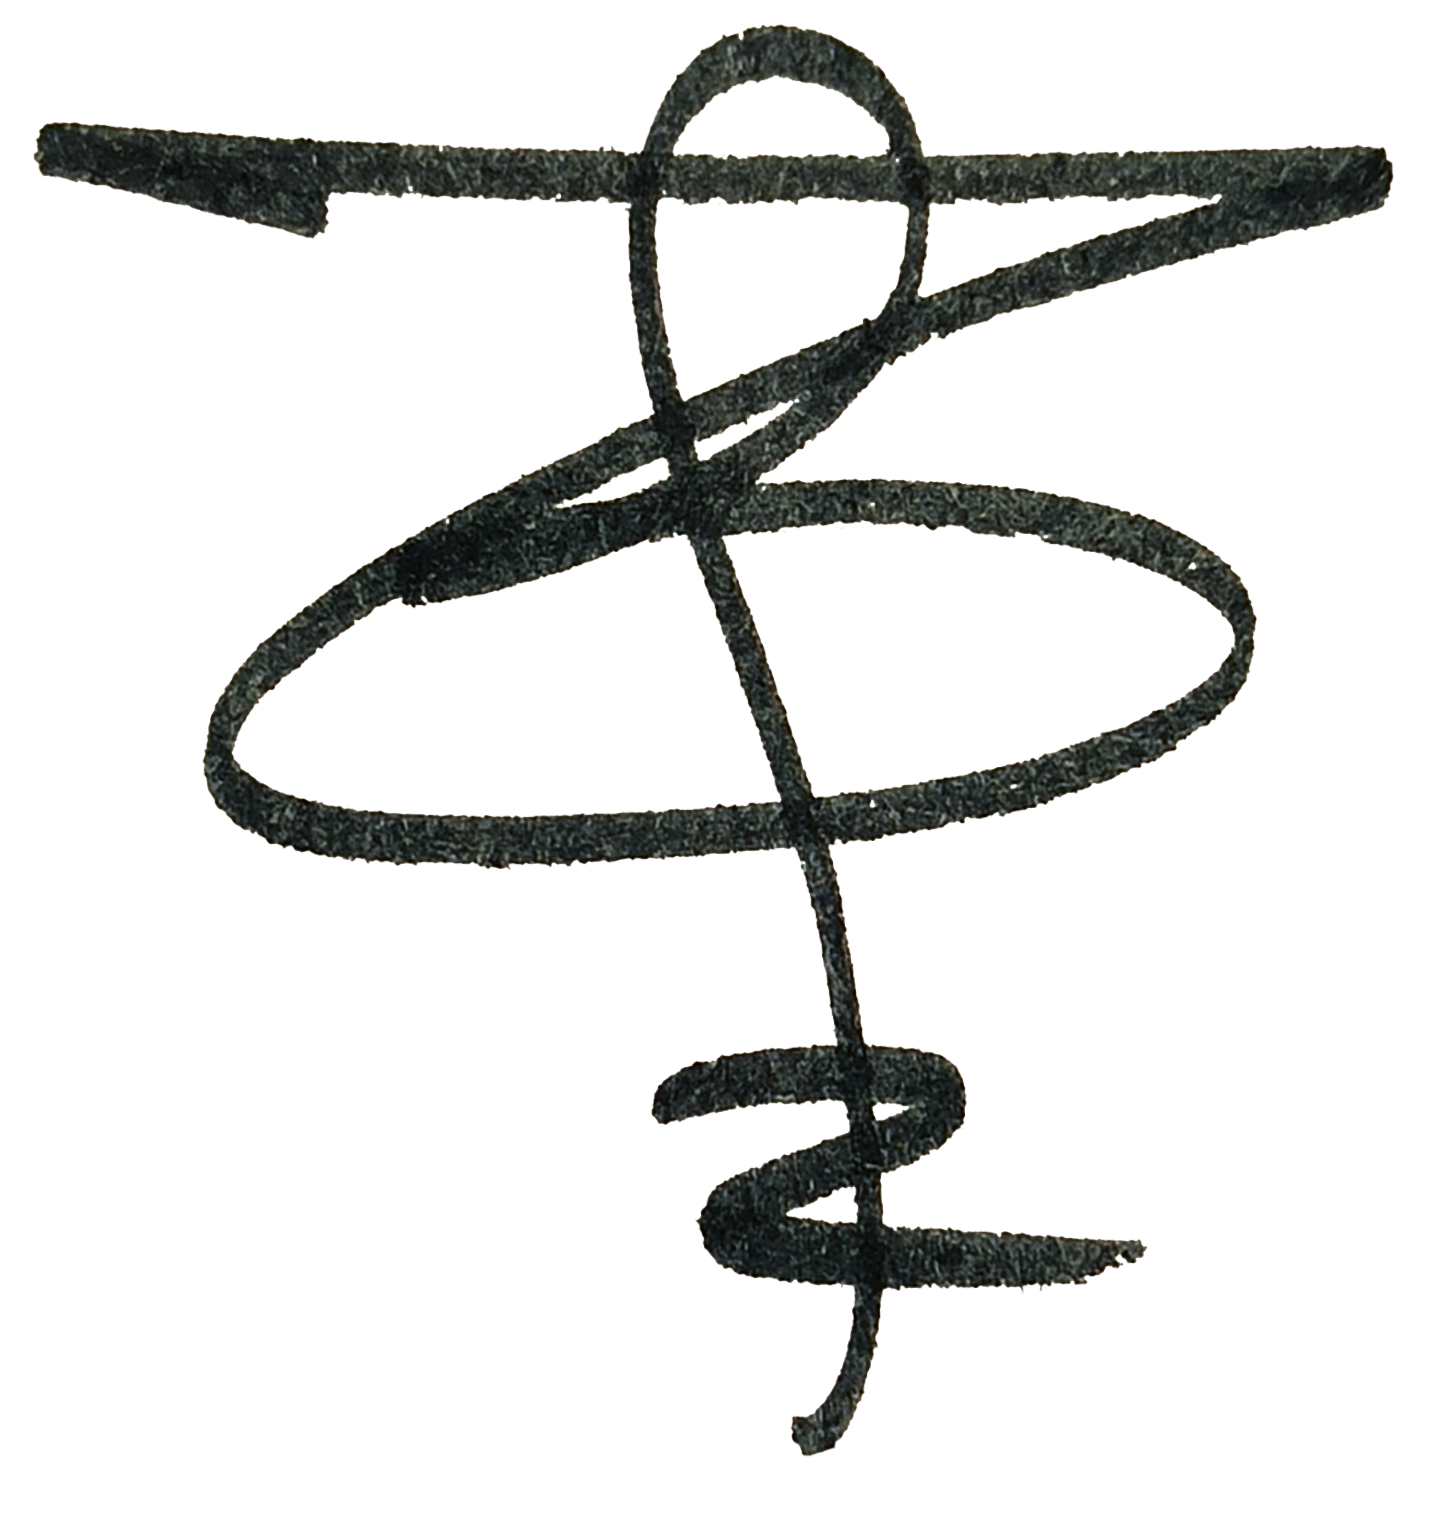
\includegraphics[height=1.7cm]{sign}};
} \end{center}}

% номер картинки, ФИО, задачи, письменно, устно

\certOnline{3}{Бойцов Денис}{50,7}{33}{5,368}
\certOnline{1}{Ушаков Дмитрий}{182,7}{28}{9,85}
\certOnline{2}{Бакланов Кирилл}{87,6}{42}{6,055}
\certOnline{1}{Несмиян Илья}{153,5}{33}{10,8}
\certOnline{2}{Басманов Денис}{79,6}{30}{7,169}
\certOnline{1}{Ширвинский Лев}{98,7}{29}{10,225}
\certOnline{2}{Скигина Жанна}{87,8}{31}{8,962}
\certOnline{1}{Кравченко Максим}{249,8}{53}{12,000}
\certOnline{2}{Гладков Денис}{100,8}{29}{8,649}
% \certOnline{}{Гвозденко Леонид}{92,4}{}{}
% \certOnline{3}{Волконская Екатерина }{23,0}{}{}

\end{document}
